
\documentclass[aps,pre,twocolumn,superscriptaddress]{revtex4-1}


\bibliographystyle{apsrev4-1}
\usepackage[colorlinks,linkcolor=blue,anchorcolor=blue,citecolor=blue,urlcolor=blue]{hyperref}


\usepackage{bm}
\usepackage{graphicx}
\usepackage{hyperref}
\usepackage{eucal}
\usepackage{amsmath}
\usepackage[capitalise]{cleveref}
\usepackage{wasysym}
\usepackage[toc,page]{appendix}


\begin{document}


\title{
Generation of plasma zonal flow shear by finite parallel wave length density fluctuations in slab geometry
}


\author{Y. Lang}
\author{Z.B. Guo}
\email[E-mail:]{ylang@pku.edu.cn}
\affiliation{
School of Physics and State Key Lab of Nuclear Physics and Technology, 
Peking University, Beijing 100871, China
}

\date{\today}


\begin{abstract}
A possible zonal flow shear generation mechanism by drift wave turbulence in a cylindrical magnetized plasma with large relative density fluctuations is discussed. These fluctuations would introduce nonlinear terms in the vorticity equation other than the term related to Reynolds stress in Hasegawa-Wakatani equations. We show that a nonlinear term can explain the generation of zonal flow in a simulation of a linear magnetized plasma device. The simulated growth of zonal flow and profile of time-averaged Reynolds stress is compared to experimental observations. We thus show that in these experiments, when the relative density fluctuation is large, Reynolds force may not be the only mechanism for zonal flow generation.
\end{abstract}
\maketitle


\section{\label{sec:introduction}introduction}


For the theoretical analysis and simulation studies, we use exactly the same model as in \cite{PhysRevE.100.033212}, except doubling the perpendicular spacial resolution 
for a more accurate analysis. In the absence of viscosity and ion-neutral collision, the vorticity equation for the plasma confined by uniform magnetic field $B\hat{\bm{z}}$ 
is $\nabla\cdot\bm{j}_{pol}+\nabla_{\parallel}j_{\parallel}=0$, i.e.
\begin{equation}
	\frac{ec}{B\Omega_{i}}\nabla\cdot\left(nd_{t}\nabla_{\perp}\phi\right)
=\nabla_{\parallel}j_{\parallel}~.
\label{eq:continuity}
\end{equation}
Where $d_{t}\equiv\partial_{t}+\bm{v}_{E}\cdot\nabla$ is the total time derivative and $\Omega_{i}\equiv eB/\left(m_{i}c\right)$ is the ion gyro-frequency. The Boussinesq approximation \cite{Ricci_2012} can be used to simplify the divergence of perpendicular current
\begin{equation}
	\nabla\cdot\left(nd_{t}\nabla_{\perp}\phi\right)=nd_{t}\nabla_{\perp}^{2}\phi~,
\label{eq:Boussinesq}
\end{equation}
which allows us to define vorticity by
\begin{equation}
	w\hat{\bm{z}}\equiv\nabla\times\bm{v}_{E}
	=\frac{c}{B}\nabla_{\perp}^{2}\phi\hat{\bm{z}}~.
\end{equation}
The vorticity equation \Cref{eq:continuity} is thus
\begin{equation}
	\partial_{t}w=-\bm{v}_{E}\cdot\nabla w
	+\frac{\Omega_{i}}{e}\frac{1}{n}\nabla_{\parallel}j_{\parallel}~.
\label{eq:vorticity}
\end{equation}


We use periodic parallel boundary condition and define the zonal-average of a given scalar field $f$ by $\left<f\right>\equiv\int_{0}^{L_{\parallel}}\int_{0}^{2\pi}f
\left(r,\theta,z\right)d\theta dz$ and perturbation by $\delta f\equiv f-\left<f\right>$. Taking zonal average of \Cref{eq:vorticity}, the LHS becomes
\begin{equation}
\begin{aligned}
	\left<\partial_{t}\nabla_{\perp}^{2}\phi\right>
&=\partial_{t}\left[\frac{1}{r}\partial_{r}
\left(r\left<v_{E,\theta}\right>\right)\right]\equiv S^{\dagger} \\
&\approx\partial_{t}\left(\partial_{r}\left<v_{E,\theta}\right>\right)\equiv S~.
\label{eq:S}
\end{aligned}
\end{equation}
In the second step we use the approximation $\partial_{r}\gg 1/r$, so this term becomes the evolution of zonal flow (ZF) shear. The first term on the RHS becomes 
\begin{equation}
\begin{aligned}
	\left<-\bm{v}_{E}\cdot\nabla w\right>
	&=-\partial_{r}\left<v_{E,r}\frac{1}{r}\partial_{r}
	\left(rv_{E,\theta}\right)\right>\equiv F_{\perp}^{\dagger} \\
	&\approx-\partial_{rr}^{2}\left<v_{E,r}v_{E,\theta}\right>\equiv F_{\perp}~,
\label{eq:Fperp}
\end{aligned}
\end{equation}
where in the second step we use the approximation $\partial_{r}\gg 1/r$ for two times, and yield the radial derivative of Reynolds' force. This drive of ZF shear has been diagnosed in many experiments \cite{doi:10.1063/1.2985836,PhysRevLett.96.195002,PhysRevLett.104.065002} through the Reynolds' stress calculated using floating potential 
\begin{equation}
	\phi_{f}=\phi-\Lambda T_{e}~,
\label{eq:phif}
\end{equation}
where $\Lambda$ is the sheath potential coefficient.


The last term in \Cref{eq:vorticity} won't be canceled by zonal average, so it is also a possible drive of ZF shear. To study its physical meaning and properties, we decompose $j_{\parallel}$ using the balance of parallel pressure drop, parallel potential drop and collision, 
\begin{equation}
j_{\parallel}=\frac{e}{\nu_{e}m_{e}}\left(\nabla_{\parallel}p_{e}-en\nabla_{\parallel}\phi\right)~.
\label{eq:Ohm}
\end{equation}
Large parallel heat conduction leads to $\nabla_{\parallel}T_{e}/T_{e}\ll\nabla_{\parallel}n/n$, so for \Cref{eq:vorticity} we have
\begin{equation}
\begin{aligned}
	F_{\parallel}^{\dagger}
	&\equiv\frac{\Omega_{i}}{e}\left<\frac{1}{n}
	\nabla_{\parallel}j_{\parallel}\right> \\
	&\approx\frac{\Omega_{i}}{m_{e}}\left<\frac{1}{n}\nabla_{\parallel}
	\left[\frac{T_{e}}{\nu_{e}}\left(\nabla_{\parallel}n-en\frac{\nabla_{\parallel}
	\phi}{T_{e}}\right)\right]\right>~.
\label{eq:Fpar_dagger}
\end{aligned}
\end{equation}
Since $\delta n$ and $\delta T_{e}$ are usually in phase, the above approximation would result in a slight loss of total amplitude. In the lowest order of $F_{\parallel}^{\dagger}$, the remaining perturbations are $\nabla_{\parallel}\delta n$, $\nabla_{\parallel}\delta\phi$ and $\delta\left(1/n\right)$. Neglecting $\delta\left(T_{e}/\nu_{e}\right)$, we define an approximation of $F_{\parallel}^{\dagger}$ by
\begin{equation}
	F_{\parallel}\equiv\frac{\Omega_{i}}{m_{e}}\left<\frac{T_{e}}{\nu_{e}}\right>
	\left<\frac{1}{n}\nabla_{\parallel}
	\left(\nabla_{\parallel}n-en\frac{\nabla_{\parallel}
	\phi}{T_{e}}\right)\right>~.
\label{eq:Fpar}
\end{equation}
For density and potential perturbations of collisional drift wave (CDW) in linear devices, the amplitude $\left|\delta\phi/T_{e}\right|/\left|\delta n/n\right|\apprle 1$ and the cross-phase $\xi\left(\tilde{n},\tilde{\phi}\right)<\pi/4$ \cite{Thakur_2014,doi:10.1063/1.1694135}. Consequently, for weakly adiabatic electrons, one would expect a secondary change of $F_{\parallel}$ if $\nabla_{\parallel}\phi$ is neglected
\begin{equation}
	F_{\parallel}\approx G_{\parallel}
	\equiv \frac{\Omega_{i}}{m_{e}}\left<\frac{T_{e}}{\nu_{e}}\right>
	\left<\left(\frac{\nabla_{\parallel}n}{n}\right)^{2}\right>~.
\label{eq:Gpar}
\end{equation}
A typical shear flow growth phase of CSDX is shown in \Cref{fig:acc_den_drive}, revealing that our approximations in \Cref{eq:Fpar_dagger,eq:Fpar,eq:Gpar} are basically valid, especially for $r<3$ cm, where perturbations are much smaller than the corresponding zonal component.
\begin{figure}[htb]
	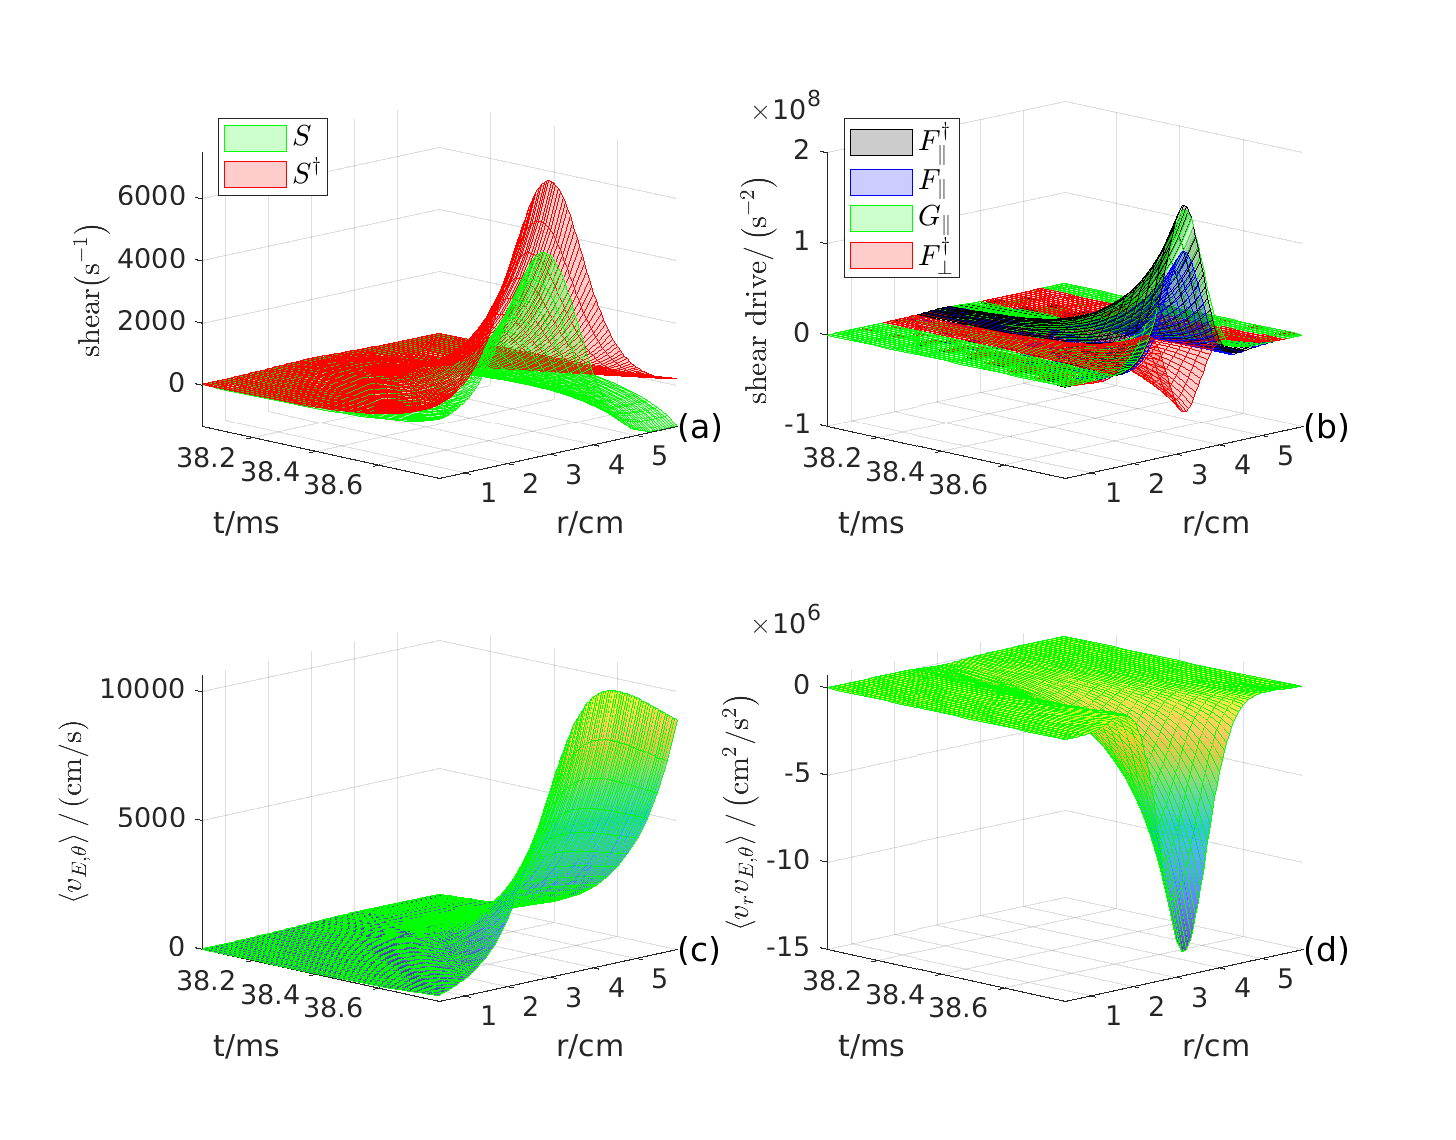
\includegraphics[width=3.375 in]{acc_den_drive.eps}
	\caption{
		Simulation result of some zonal-averaged fields in a typical shear flow growth phase. (a) evolution of flow shear, defined in \Cref{eq:S}. (b) evolution of flow shear drives, defined in \Cref{eq:Fperp,eq:Fpar_dagger,eq:Fpar,eq:Gpar}.
		\label{fig:acc_den_drive}	
	}
\end{figure}


As can be seen in \Cref{fig:acc_den_drive}(a), the flow shear grows globally, with the maximum amplitude near $r\approx 3$ cm, where $\left<n\right>$ and $\left<T_{e}\right>$ has the maximum gradient, and the instability has the maximum intensity. \Cref{fig:acc_den_drive}(b) shows that, the main drive of zonal flow shear is $F_{\parallel}^{\dagger}$, and $F_{\perp}^{\dagger}$flattens the flow profile. The resulting growth of $\bm{E}\times\bm{B}$ is shown in \Cref{fig:acc_den_drive}(c), which can be compared to time-delay estimation (TDE) results in \cite{PhysRevLett.104.065002,doi:10.1063/1.3322823}. Note that the TDE result would include CDW phase velocity as explained in \cite{PhysRevE.100.033212}. Reynolds' stress can be regarded as ZF flux, peaking near the maximum ZF shear location (\Cref{fig:acc_den_drive}(d)), convecting ZF down its gradient. \Cref{eq:Gpar} shows that, the main part of $F_{\parallel}^{\dagger}$, $G_{\parallel}$, is positive definite. At the edge of tokamaks where $\nu_{e}$ is relatively high, the relatively weakly adiabatic electrons would hardly cancel $G_{\parallel}$, so there should always be a finite drive of positive $E_{r}$ shear. 


As a validation of our simulation, we compare our simulation result of Reynolds' stress with experimental observations. For the argon plasma in CSDX, the sheath potential coefficient in \Cref{eq:phif} is estimated by \cite{Nie_2018}
\begin{equation}
	\Lambda=\frac{1}{2}\ln\left(\frac{m_{i}}{2\pi m_{e}}\right)\approx 4.68~,
\label{eq:Lamda}
\end{equation}
which is significantly larger than deuterium plasmas, making the approximation $\phi\approx\phi_{f}$ easier to break down. The breaking in our simulation is shown in \Cref{fig:comp_pl_fl}. In spite of a somewhat unknown filter used in experiments, our simulation results of time-averaged synthetic $\left<v_{E,r}v_{E,\theta}\right>$ and $\left<v_{E,r}^{2}\right>$ agree with experimental observations well \cite{doi:10.1063/1.2985836,PhysRevLett.104.065002}. However, when we use plasma potential $\phi$, the amplitude of the two profiles reduce significantly, and the Reynolds' stress changes shape.

\begin{figure}[htb]
	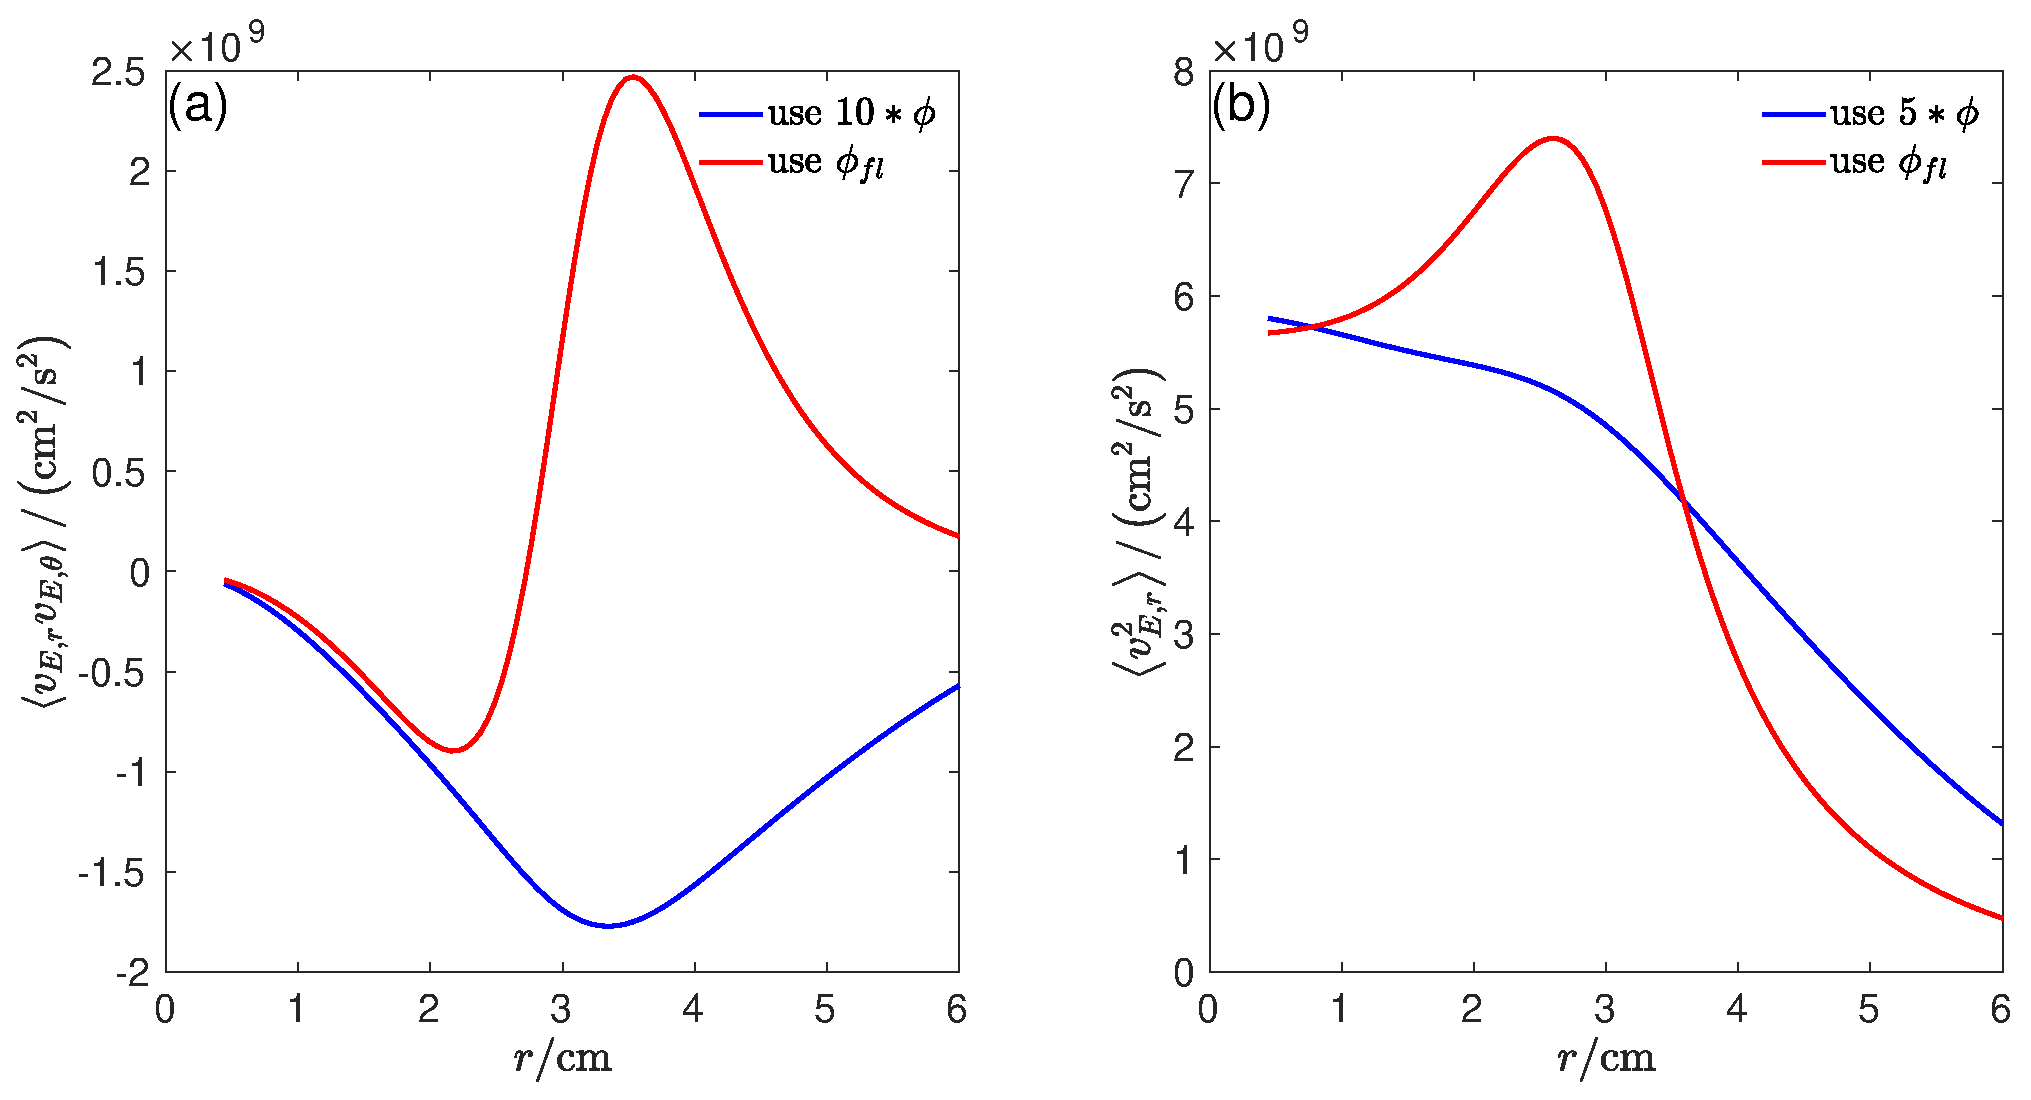
\includegraphics[width=3.375 in]{comp_pl_fl.eps}
	\caption{
		Simulation result of some zonal and time averaged fields during $t=9.4-50.8$ ms. The blue curves are calculated using multiples of plasma potential, while the red curves are calculated using synthetic floating potential given by \Cref{eq:phif,eq:Lamda}. (a) Reynolds' stress and (b) the intensity of radial $\bm{E}\times\bm{B}$ velocity perturbations.
		\label{fig:comp_pl_fl}	
	}
\end{figure}


\bibliography{ZF.bib}



\end{document}

